\documentclass[12pt]{article}
\usepackage{amsmath}
\usepackage{listings}
\usepackage{color}
\usepackage{geometry}
\usepackage{float} % Required for the [H] float option
\usepackage{graphicx} % Required for including images
\geometry{margin=1in}
\usepackage{caption}
\usepackage[colorlinks=true, linkcolor=black, urlcolor=blue, citecolor=blue]{hyperref}
\usepackage{fancyhdr}
\usepackage{color}
\usepackage{xcolor} % Needed for custom colors
\definecolor{purple}{rgb}{0.5,0.0,0.5} % Define purple manually
\definecolor{codegray}{rgb}{0.5,0.5,0.5}
\definecolor{backcolour}{rgb}{0.95,0.95,0.92}


\pagestyle{fancy}
\fancyhead[L]{ Assignment -2 }
\fancyhead[R]{Gandholi Sarat - 23008}
\title{\textbf{PMAT 402 - Systems Programming \\ Assignment -2 \\ SIC/XE Instruction Parser}}
\author{\textbf{Gandholi Sarat - 23008}}
\author{Gandholi Sarat - 23008}
\date{April 10, 2025}

\definecolor{codegray}{rgb}{0.5,0.5,0.5}
\definecolor{backcolour}{rgb}{0.95,0.95,0.92}
\lstdefinestyle{mystyle}{
    backgroundcolor=\color{backcolour},   
    commentstyle=\color{codegray},
    keywordstyle=\color{blue},
    numberstyle=\tiny\color{codegray},
    stringstyle=\color{purple},
    basicstyle=\ttfamily\footnotesize,
    breakatwhitespace=false,         
    breaklines=true,                 
    captionpos=b,                    
    keepspaces=true,                 
    numbers=left,                    
    numbersep=5pt,                  
    showspaces=false,                
    showstringspaces=false,
    showtabs=false,                  
    tabsize=2
}
\lstset{style=mystyle}

\begin{document}

\renewcommand{\thesection}{\Roman{section}}
\renewcommand{\thesubsection}{\Roman{section}.\Roman{subsection}}

\maketitle
\tableofcontents
\newpage

\section{Objective}

The objective of this program is to implement a C++ class that parses SIC (Simplified Instructional Computer) instructions and extracts key components from them. The program takes a hexadecimal SIC instruction (either 6 or 8 digits) as input and performs the following tasks:

\begin{itemize}
    \item \textbf{Fetch Opcode:} Extract the 6-bit operation code using the \texttt{getOpcode()} function.
    \item \textbf{Extract Flags (nixbpe):} Retrieve the six control bits using the \texttt{getFlags()} function, which represent addressing and format options.
    \item \textbf{Determine Addressing Mode:} Analyze the flags to identify whether the instruction uses immediate, indirect, indexed, base-relative, PC-relative, or direct addressing via the \texttt{getAddressingMode()} function.
    \item \textbf{Compute Displacement Address:} Calculate the memory address involved in the instruction using the \texttt{getDispAddr()} function.
    \item \textbf{Identify Instruction Format:} Determine whether the instruction uses Format 3 or Format 4 by examining the \texttt{e} flag via the \texttt{getFormat()} function.
\end{itemize}


\section{Code Listing}
\begin{lstlisting}[language=C++,caption={SIC Instruction Parser in C++}]
    #include <iostream>
    #include <bitset>
    #include <string>
    #include <sstream>
    #include <iomanip>
    #include <cstdint>
    
    class MyParse {
        public:  // Make the function public
            // Convert hex string to 32-bit unsigned integer
            uint32_t hexTo32BitUnsigned(const std::string& hexInput) {
                uint32_t value;
                std::stringstream ss;
                ss << std::hex << hexInput;
                ss >> value;
    
                if (hexInput.length() == 6) {
                    // Append zeros by shifting left 8 bits
                    uint32_t value32Bit = value << 8;
                    return value32Bit;
                } 
                else if (hexInput.length() == 8) {
                    // Already a 32-bit value
                    return value;
                } 
                else {
                    // Invalid input length
                    std::cerr << "Invalid input: Please provide either 6 or 8 hexadecimal digits." << std::endl;
                    return 0;  // Returning 0 for invalid inputs
                }
            }
    
            // Extract opcode (6 bits) from binary instruction
            std::bitset<6> getOpcode(uint32_t binary){
                uint32_t opcode = (binary >> 26) & 0x3F;
                return std::bitset<6> (opcode);
            }
    
            // Extract flags (nixbpe) from binary instruction
            std::bitset<6> getFlags (uint32_t binary){
                uint32_t flags = (binary >> 20) & 0x3F;
                return std::bitset<6> (flags);
            }
            
            // Determine addressing mode based on flags
            std::string getAddressingMode(std::bitset<6> flags){
                if (!flags[5] && flags[4] && !flags[3] )
                    return "Immediate Addressing Mode";
                if (flags[5] && !flags[4] && !flags[3] )
                    return "Indirect Addressing Mode";
                if (flags[3] && !flags[2] && !flags[1] )
                    return "Index Addressing Mode";
                if (flags[2] && !flags[1] )
                    return "Base Relative Addressing Mode";
                if (!flags[2] && flags[1] )
                    return "Program-Counter Relative Addressing Mode";
                if (!flags[2] && !flags[1] )
                    return "Direct Addressing Mode";
                else
                    return "Unknown Addressing Mode";	
            }
    
            // Compute Displacement address based on flags and hex input
            std::bitset<20> getDispAddr(const std::string& hexInput) {
                uint32_t value = hexTo32BitUnsigned(hexInput);
                auto flags = getFlags(value);
    
                uint32_t DisplacementAddress = 0;
    
                if (flags[0]) { // Format 4: Use 20-bit Displacement address
                    DisplacementAddress = value & 0xFFFFF;  // Mask to get the lower 20 bits
                } 
                else { // Format 3: Use 12-bit Displacement address
                    DisplacementAddress = value & 0xFFFFF;  // Mask to get the lower 12 bits
                }
    
                // Return the Displacement address as a 20-bit bitset
                return std::bitset<20>(DisplacementAddress);
            }
    
            // Determine instruction format (3 or 4) based on flags
            unsigned int getFormat(std::bitset<6> flags) {
                return flags[0] ? 4 : 3;  // Format 4 if e-bit is set, else Format 3
            }
    };
    
    int main() {
        MyParse parser;
    
        // Take input from user
        std::string hexInput;
        std::cout << "Enter a hexadecimal instruction (6 or 8 characters): ";
        std::cin >> hexInput;
    
        // Validate input length
        if (hexInput.length() != 6 && hexInput.length() != 8) {
            std::cerr << "Error: Invalid input length. Please provide either 6 or 8 hexadecimal digits." << std::endl;
            return 1; // Exit with error code
        }
    
        // Convert hex input to binary
        uint32_t binary = parser.hexTo32BitUnsigned(hexInput);
    
        // Extract and display opcode
        auto opcode = parser.getOpcode(binary);
        std::cout << "Opcode: " << opcode << "\n";
    
        // Extract and display flags (nixbpe)
        auto flags = parser.getFlags(binary);
        std::cout << "Flags (nixbpe): " << flags << "\n";
    
        // Determine and display addressing mode
        auto addressingMode = parser.getAddressingMode(flags);
        std::cout << "Addressing Mode: " << addressingMode << "\n";
    
        // Compute and display display address
        auto DisplacementAddress = parser.getDispAddr(hexInput);
        std::cout << "Disp Address: " << DisplacementAddress << "\n";
    
        // Determine and display instruction format
        auto format = parser.getFormat(flags);
        std::cout << "Instruction Format: " << format << "\n";
    
        return 0;
    }
\end{lstlisting}

\section{Code Output}
\begin{verbatim}
Enter a hexadecimal instruction (6 or 8 characters): 032600
Opcode: 000000
Flags (nixbpe): 110010
Addressing Mode: Program-Counter Relative Addressing Mode
Disp Address: 01100000000000000000
Instruction Format: 3

Enter a hexadecimal instruction (6 or 8 characters): 03C300
Opcode: 000000
Flags (nixbpe): 111100
Addressing Mode: Base Relative Addressing Mode
Disp Address: 00110000000000000000
Instruction Format: 3

Enter a hexadecimal instruction (6 or 8 characters): 022030
Opcode: 000000
Flags (nixbpe): 100010
Addressing Mode: Indirect Addressing Mode
Disp Address: 00000011000000000000
Instruction Format: 3

Enter a hexadecimal instruction (6 or 8 characters): 010030
Opcode: 000000
Flags (nixbpe): 010000
Addressing Mode: Immediate Addressing Mode
Disp Address: 00000011000000000000
Instruction Format: 3

Enter a hexadecimal instruction (6 or 8 characters): 003600
Opcode: 000000
Flags (nixbpe): 000011
Addressing Mode: Program-Counter Relative Addressing Mode
Disp Address: 01100000000000000000
Instruction Format: 4

Enter a hexadecimal instruction (6 or 8 characters): 0310C303
Opcode: 000000
Flags (nixbpe): 110001
Addressing Mode: Direct Addressing Mode
Disp Address: 00001100001100000011
Instruction Format: 4
\end{verbatim}


\section{Output comparison}
\begin{figure}[H]
    \centering
    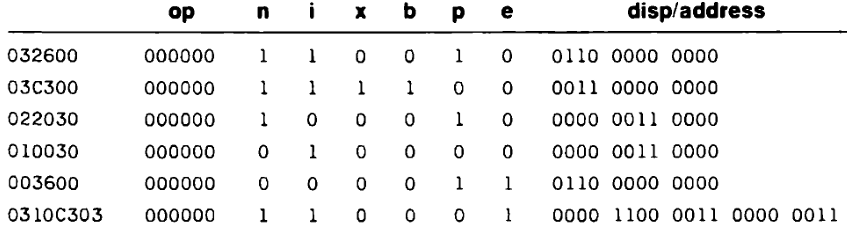
\includegraphics[width=0.8\textwidth]{Sample.png}
    \caption{Expected ouput, Table from textbook} 
    \label{fig:output}
\end{figure}
The output of the program is consistent with the expected results from textbook for various SIC instructions. The opcode, flags, addressing mode, displacement address, and instruction format are accurately extracted and displayed based on the provided hexadecimal input.

\section{Function Descriptions}

\subsection{hexTo32BitUnsigned}
Converts a 6- or 8-digit hexadecimal string into a 32-bit unsigned integer. If the input is 6 digits, it shifts the value left by 8 bits to simulate 24-bit instructions.

\subsection{getOpcode}
Extracts the first 6 bits from the most significant end of the instruction to retrieve the opcode.

\subsection{getFlags}
Extracts the \texttt{nixbpe} flags from bits 20-25 of the 32-bit instruction.

\subsection{getAddressingMode}
Determines the addressing mode using the flags:
\begin{itemize}
    \item \textbf{Immediate:} \texttt{n=0, i=1}
    \item \textbf{Indirect:} \texttt{n=1, i=0}
    \item \textbf{Index:} \texttt{x=1}
    \item \textbf{Base-relative:} \texttt{b=1, p=0}
    \item \textbf{PC-relative:} \texttt{b=0, p=1}
    \item \textbf{Direct:} \texttt{b=0, p=0}
\end{itemize}

\subsection{getDispAddr}
Computes the Displacement address:
\begin{itemize}
    \item For Format 4 (e=1), uses a 20-bit address.
    \item For Format 3 (e=0), masks similarly to maintain 12-bit Displacement addressing.
\end{itemize}

\subsection{getFormat}
Returns the instruction format:
\begin{itemize}
    \item Format 3: if \texttt{e = 0}
    \item Format 4: if \texttt{e = 1}
\end{itemize}



\end{document}
